\section{Month 1 - May}

\subsection{Initial Approach}

To begin this project, we will investigate different ways to utilize GPU graphics cards for the parallel processing of numerical calculation codes. There are several options available for the development of this task, but the proposal is to combine Python for creating the user interface and the use of Fortran and C++ for the numerical problem itself.

We aim to achieve results as good as those from Matlab using the GPU. We can see the results obtained in some benchmarks for Matlab below:

\begin{center}
\begin{figure}[H]
\centering
\begin{minipage}[b]{0.32\linewidth}
\centering
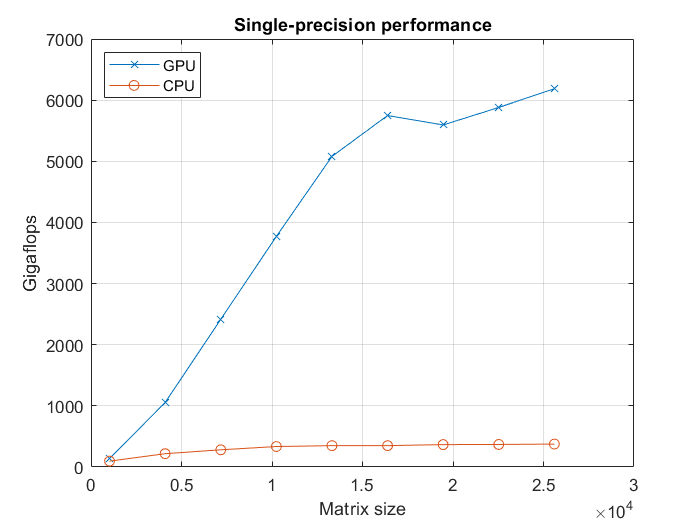
\includegraphics[width=\linewidth]{Figures/Imagenes/single.png}
\caption{}
\end{minipage}
\begin{minipage}[b]{0.32\linewidth}
\centering
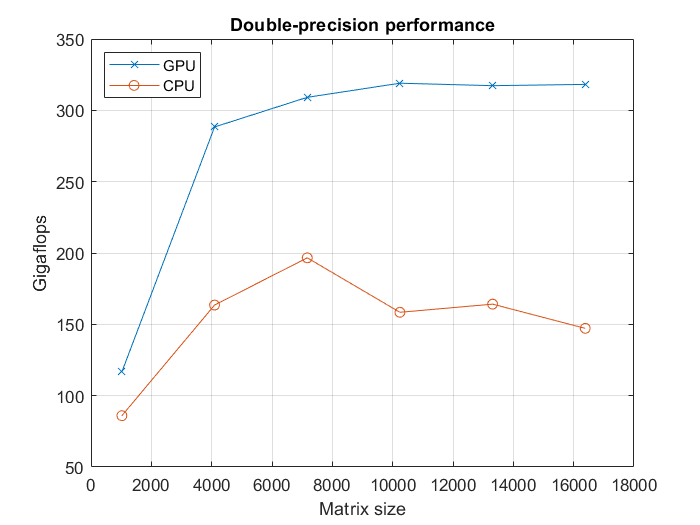
\includegraphics[width=\linewidth]{Figures/Imagenes/double.png}
\caption{}
\end{minipage}
\begin{minipage}[b]{0.32\linewidth}
\centering
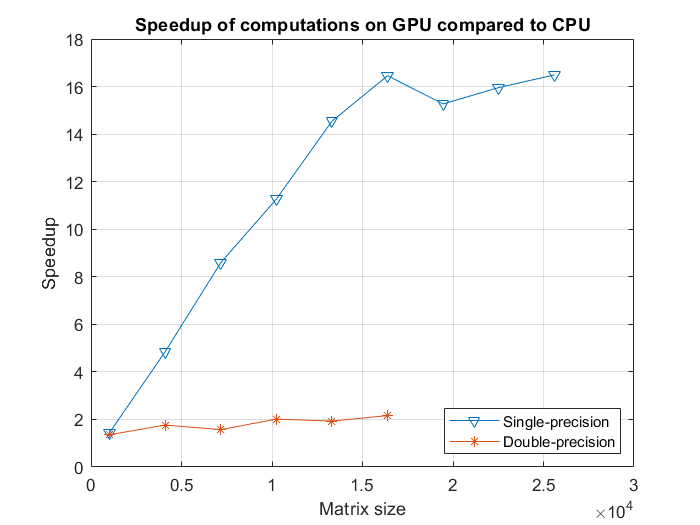
\includegraphics[width=\linewidth]{Figures/Imagenes/speedup.png}
\caption{}
\end{minipage}
\end{figure}
\end{center}

\vspace{-1em}

We can observe that performance under single precision (Figure 1) skyrockets when we use the GPU versus the CPU, we see this is not the case for double precision (Figure 2). In Figure 3, we see a relationship between the performance achieved with the GPU vs. the CPU where we see that the larger the matrix dimension, this ratio increases, seeing results up to 16 times better with the GPU than with the CPU.



\subsection{Python Benchmark (CuPy) code}

To begin with, this first week I will be creating a script of a benchmark for CuPy, comparing its performance to NumPy in the context of matrix-vector multiplication operations. 
We can see the code of the operations below:

\begin{lstlisting}
    print("\nComparing performance for dimension N = {}\n".format(dim))
    
    np_matrix = np.empty((dim, dim), dtype=np.float32)
    np_vector = np.empty(dim, dtype=np.float32)
    numpy_random_matrix(dim, np_matrix)
    numpy_random_vector(dim, np_vector)
    
    start = time.time()
    for i in range(10000):
    
         numpy_result = i*numpy_dot(np_matrix, np_vector)

    numpy_time = time.time() - start


    cp_matrix = cp.empty((dim, dim), dtype=cp.float32)
    cp_vector = cp.empty(dim, dtype=cp.float32)
    cupy_random_matrix(dim, cp_matrix)
    cupy_random_vector(dim, cp_vector)

    start = time.time()
    for i in range(10000):

        cupy_result = i*cupy_dot(cp_matrix, cp_vector)
   
    cupy_time = time.time() - start

    start = time.time()

    np_cupy_result = cp.asnumpy(cupy_result)
    cupy_transfer_time = time.time() - start
    
\end{lstlisting}

\subsection{Why we don't get any better than 15x-20x performance with the GPU}


Modern x86-64 Intel/AMD processor can generally compute 2 (256 AVX) SIMD vectors in parallel since there is generally 2 SIMD units. Processors like Intel Skylake also have 4 ALU units capable of computing 4 basic arithmetic operations (eg. add, sub, and, xor) in parallel per cycle. This can significantly speed up certain operations, especially in tasks like image processing and game physics where the same operations often need to be performed on large sets of data.


To illustrate this comparison further, we can look at the AMD Ryzen 5 5600X CPU. This 6-core processor has 2x256 bit SIMD units per core. This CPU can manage instructions with up to a 512 bit vector as we said before.

\clearpage

However, NVIDIA GPUs execute groups of threads known as warps in SIMT (Single Instruction, Multiple Thread) fashion. In this case, one instruction can operate 32 items in parallel (Remeber, this is theoretically, hardware can be free not to do that completely in parallel). Knowing this, we can consider a CPU core equivalent to ``16 CUDA cores'' (512/32 = 16). Therefore, a Ryzen 5 5600X would have the equivalent to $6 \cdot 16 = 96$ ``CUDA cores''.

We also computed the ratio of the number of CUDA cores in the RTX 3070 (5,888 CUDA cores) to the number of ``CUDA cores'' in the Ryzen 5 5600X:

\vspace{-0.5em}
\begin{center}
$\dfrac{{5888}}{{96}} = 61.33$
\end{center}

This indicates that the GPU has approximately 61.33 times as many CUDA cores as the CPU.

However, we must also consider the clock speeds of the GPU and CPU, which are 1.4 GHz and 4.6 GHz, respectively. Taking this into account, we find that the potential speedup of the GPU compared to the CPU is approximately:

\begin{center}
$\dfrac{{61.33 * 1.4}}{{4.6}} \approx 18.58$.
\end{center}

It's important to understand that these comparisons greatly oversimplify the architectural differences between CPUs and GPUs. They are mainly illustrative and should not be used to predict performance across different types of tasks.


\clearpage

\subsection{Benchmarks repository v1}

Our goal for this week is to create a benchmark repository for Python, Fortran, C, and Matlab. The purpose of this benchmark repository is to compare the execution time of the same operation across these different programming languages.

To recap, in week 1, we performed a particular operation in Python. This week, we will replicate that operation in Fortran, C, and Matlab. By doing so, we can measure and compare the time it takes for each language to perform the same task. This will provide us with useful insights into the relative performance of these languages.

\vspace{1em}


\begin{table}[h]
\resizebox{\textwidth}{!}{%
\begin{tabular}{|c|c|c|c|c|c|c|}
\hline
N                      & \textbf{CPU}              & \textbf{GPU}              & \textbf{Test} & \textbf{CPU (SC) Time} & \textbf{CPU (MC) Time} & \textbf{GPU Time} \\ \hline
\multirow{4}{*}{5000}  & \multirow{4}{*}{R5 5600X} & \multirow{4}{*}{RTX 3070} & Matlab        & 289.03s                & 181.21s                & 8.28s             \\ \cline{4-7} 
                       &                           &                           & Python        & NA                     & 26.41s                 & 2.45s             \\ \cline{4-7} 
                       &                           &                           & Fortran       &                        &                        &                   \\ \cline{4-7} 
                       &                           &                           & C++           & 767.82s                & 101.73s                 &                   \\ \hline
\multirow{4}{*}{10000} & \multirow{4}{*}{R5 5600X} & \multirow{4}{*}{RTX 3070} & Matlab        & 1087.51s               & 637.95s                & 30.24s            \\ \cline{4-7} 
                       &                           &                           & Python        & NA                     & 162.15s                & 9.52s             \\ \cline{4-7} 
                       &                           &                           & Fortran       &                        &                        &                   \\ \cline{4-7} 
                       &                           &                           & C++           &                        &                        &                   \\ \hline
\end{tabular}%
}
\end{table}


Remember that this is a preliminary approach and our first contact with the benchmarks. It serves as a starting point for identifying areas of improvement.


\subsection{Optimizing CPU Utilization with Vectorization}

In light of the performance issues experienced in our single-core benchmarks, our primary focus this week is shifting from GPU parallelization to optimizing CPU utilization. In particular, we will be forcing vectorization to take advantage of SIMD (Single Instruction, Multiple Data) instructions and standards such as AVX2/256bits on my Ryzen 5 5600X

As we have observed from the benchmark test results, in some laguages we are not using 100\% of CPU capacity. One potential reason could be the lack of vectorization in our code. Vectorization is a critical aspect of numerical computation which allows a processor to perform a single operation on multiple data points simultaneously. This can significantly improve the execution speed of our programs.

\clearpage

\subsection{Vectorization in Different Programming Languages}

\subsubsection*{Matlab}
Matlab is inherently good at vectorized operations due to its matrix-based design. It will automatically use vectorization when possible. This is why we got great results without doing any tweak. This was our goal with the rest of languages.

\subsubsection*{Python:} Python, with libraries such as NumPy, can perform vectorized operations efficiently. NumPy arrays can significantly speed up the operations by implicitly allowing element-wise operations. Vectorization here is implicit and does not require any special syntax to enable it. This is due to NumPy's design to handle array operations efficiently by performing element-wise operations on arrays.

However, to ensure that you are taking advantage of vectorization, you should:

\begin{itemize}[label={\scriptsize\raisebox{0.5ex}{\textbullet}}]

\itemsep=0.3em\topsep=0pt\partopsep=0pt
\parskip=0pt\parsep=0pt

\setitemize{leftmargin=1em}

 \item \textbf{Use NumPy's built-in functions} and operations as is optimized for array operations.

 \item \textbf{Avoid loops:} The whole point of vectorization is to eliminate explicit loops over elements in arrays.fhere may be a way to do the operation using NumPy's vectorized operations.

 \item \textbf{Broadcasting:} Understand and utilize broadcasting, a powerful mechanism that allows NumPy to work with arrays of different shapes when performing arithmetic operations. For example, you can add a scalar to an array, and NumPy will add that scalar to each element in the array.
 
\end{itemize}


\subsubsection*{Fortran:}

Intel Fortran have features for automatic vectorization. This includes the use of Single Instruction, Multiple Data (SIMD) instructions.

The Intel Fortran compiler uses various flags to enable and optimize vectorization. For instance, the \texttt{-O3} flag turns on the compiler's optimization, including vectorization.

To benefit the most from vectorization, Fortran code might need adjustments to conform to certain conditions. Some best practices include:

\begin{itemize}
\item \textbf{Loop Independence:} Each iteration of the loop should be independent; the result of an iteration should not depend on the results of other iterations.
\item \textbf{Array Operations:} Fortran naturally lends itself to array operations, which can be implicitly vectorized.
\item \textbf{Compiler Directives:} Compiler directives, such as \texttt{!DIR\$ SIMD} before a loop, can give the compiler hints to assist with vectorization.
\end{itemize}



\subsubsection*{C++:}

The Intel C++ compiler utilizes various flags to enable and guide the process of vectorization. For instance, the \texttt{-O3} flag activates the compiler's optimization, including vectorization. Furthermore, the \texttt{-xHost} flag generates instructions for the highest instruction set available on the host processor. The \texttt{-vec-report} flag can be used to get a report on vectorization decisions made by the compiler.

To fully exploit vectorization, C++ code might need to be adjusted to certain conditions:

\begin{itemize}
\item \textbf{Loop Independence:} The iterations of a loop should ideally be independent; the result of one iteration should not depend on the result of other iterations.
\item \textbf{Data Alignment:} Data should be aligned in memory for optimal performance. Many modern compilers can automatically align data, but it is possible to manually specify alignment in your C++ code.
\item \textbf{Compiler Directives:} Compiler directives or pragmas can provide additional hints to the compiler. For instance, the \texttt{\#pragma simd} directive can suggest to the compiler that a loop should be vectorized.
\end{itemize}

It is important to remember that efficient vectorization requires a deep understanding of the code and the target hardware. Always ensure the correctness of the computation after vectorization, as parallel execution can introduce numerical differences due to the reordering of operations.